\documentclass[fontsize=10pt]{scrartcl}

\usepackage{enumitem}
	\setenumerate{listparindent=\parindent}
\usepackage{amsmath}
\usepackage{amssymb}
\usepackage{graphicx}
\usepackage{placeins}
\usepackage{hyperref}
\usepackage{float}
\usepackage[hyphenbreaks]{breakurl}
\usepackage[margin=1.0in]{geometry}

\newcommand{\code}{\texttt}

\begin{document}

	\title{CSC 522 : Automated Learning and Data Analysis}
	\subtitle{Homework 4}
	\author{Roopak Venkatakrishnan - rvenkat7@ncsu.edu}
	\maketitle

	\section{Question 1}
		Kaggle \url{http://www.kaggle.com/} is a platform for predictive modeling competitions which are hosted by various agencies around the world. The recommended project for this course is one such competition. This exercise aims at introducing students to the Kaggle environment.
		

		This is the easiest question in the entire course; please don’t make a mistake. Complete the following task.

		\begin{itemize}
			\item
			Go to \url{http://www.kaggle.com/}

			\item
			If you are not a member already, signup

			\item
			Go to the Database in Moodle and enter your unity ID, Kaggle user name and Kaggle userID.
		\end{itemize}

		\textbf{Answer:} \\
		\begin{itemize}
			\item
			Unity ID - rvenkat7

			\item
			Kaggle User Name - roopakv

			\item
			Kaggle Display Name - Roopak Venkatakrishnan
		\end{itemize}


		\section{Question 2}

		For this exercise, you will use the getting started competition Titanic: Machine Learning from Disaster \url{http://www.kaggle.com/c/titanic-gettingStarted}. You may use Matlab, R or Weka. Note there is a tutorial on this contest posted on  he course website. Submissions to Kaggle are scored on the basis of classification accuracy, which is the proportion of test cases that are correctly classified. The data can be found here \url{http://www.kaggle.com/c/titanic-gettingStarted/data} and forums with a lot of helpful discussion can be found here \url{http://www.kaggle.com/c/titanic-gettingStarted/forums}. Also note that you only get two submissions to Kaggle per day, so please submit early and often to ensure you can complete this assignment. Make sure your submissions match the format provided in the tutorial to avoid wasting submission.

		Complete the following tasks.

		\begin{enumerate}
			\item
			All machine learning models have parameters that can be tuned. These parameters can either have a positive or negative effect on the performance of the algorithm. Crossvalidation (CV) is one approach to identify a good model. For each of the algorithms below, identify the set of parameters that give the best predictive performance in terms of classification accuracy. You are free to do this in whatever way you wish, but in R you might consider using the train function in the caret package to help you with 1this task. This reference may be helpful \url{http://caret.r-forge.r-project.org/training.html}

			\begin{itemize}
				\item
				A decision tree (ID3, Gini, C4.5, C5 or any other single decision tree)

				\item
				A boosted tree. Use Statistics Toolbox -> Functions -> Nonparametric Supervised Learning -> Ensemble Methods in Matlab or the gbm package in R. In R, the tuning parameters for this function are \texttt{interaction.depth} (how big each tree is), n.trees (how many trees to grow), shrinkage (a parameter to control overfitting). Weka has ensemble models as well.
			\end{itemize}

			Your answers must include at least 5 different sets of parameters that you tried. State why you changed the parameters for each set. Report the cross-validation scores for each of the 5 sets for each approach. Use k=5 for a k-way cross-validation. Note you do not have to report the Kaggle leaderboard score for each.

			\textbf{Answer:}

			\subsection{Decision Tree}

\begin{verbatim}
> vals <- read.csv(file.choose())
> Y<- as.factor(vals$survived)
> X <- data.frame(age=vals$age,
+                    fare=vals$fare,
+                    pclass=vals$pclass,
+                    sex=as.integer(factor(vals$sex)))
> X$fare[ is.na( X$fare) ] <- -1
> X$age[ is.na( X$age) ] <- -1
> thedata <- cbind(Y,X)
> cvinfo <- trainControl(method = "cv", number = 5)
> rpart_control <- expand.grid(.cp = c(0.01,0.1,.25,0.5,1)) 
> train(Y~.,data=thedata,method="rpart",trControl=cvinfo,tuneGrid=rpart_control)
891 samples
  4 predictors
  2 classes: '0', '1' 

No pre-processing
Resampling: Cross-Validation (5 fold) 

Summary of sample sizes: 713, 712, 713, 713, 713 

Resampling results across tuning parameters:

  cp    Accuracy  Kappa  Accuracy SD  Kappa SD
  0.01  0.798     0.549  0.0254       0.0568  
  0.1   0.787     0.542  0.0239       0.052   
  0.25  0.787     0.542  0.0239       0.052   
  0.5   0.616     0      0.0026       0       
  1     0.616     0      0.0026       0       

Accuracy was used to select the optimal model using  the largest value.
The final value used for the model was cp = 0.01. 
\end{verbatim}
			
			We notice that the accuracy decreases as the control value increases. Thus let us now try an use a lower set of values. We try and center the values around 01 as we noticed that we got the best accuracy for it after which it seemed to fall. We can guess that the accuracy increases till it reaches a max and then drops back down. using this information we have to try different values of cp till we find the maxima.

\begin{verbatim}
> rpart_control <- expand.grid(.cp = c(0.001,0.005,.01,.02,.05)) 
> train(Y~.,data=thedata,method="rpart",trControl=cvinfo,tuneGrid=rpart_control)
891 samples
  4 predictors
  2 classes: '0', '1' 

No pre-processing
Resampling: Cross-Validation (5 fold) 

Summary of sample sizes: 713, 713, 712, 713, 713 

Resampling results across tuning parameters:

  cp     Accuracy  Kappa  Accuracy SD  Kappa SD
  0.001  0.797     0.562  0.0395       0.0752  
  0.005  0.792     0.549  0.0354       0.0652  
  0.01   0.804     0.565  0.0105       0.0195  
  0.02   0.802     0.569  0.0136       0.0232  
  0.05   0.787     0.542  0.0262       0.0531  

Accuracy was used to select the optimal model using  the largest value.
The final value used for the model was cp = 0.01. 
\end{verbatim}

			Again we can see that the maxima is around .01 and that it slightly decreases if we move to .02. Thus the next step is to narrow down further closer to .01 and try and figure out where the maxima might be.

\begin{verbatim}
> rpart_control <- expand.grid(.cp = c(0.0095,0.0099,.01,.011,.015)) 
> train(Y~.,data=thedata,method="rpart",trControl=cvinfo,tuneGrid=rpart_control)
891 samples
  4 predictors
  2 classes: '0', '1' 

No pre-processing
Resampling: Cross-Validation (5 fold) 

Summary of sample sizes: 713, 713, 713, 713, 712 

Resampling results across tuning parameters:

  cp      Accuracy  Kappa  Accuracy SD  Kappa SD
  0.0095  0.799     0.554  0.0225       0.0531  
  0.0099  0.799     0.554  0.0225       0.0531  
  0.01    0.799     0.554  0.0225       0.0531  
  0.011   0.805     0.566  0.0192       0.0434  
  0.015   0.801     0.56   0.0241       0.0514  

Accuracy was used to select the optimal model using  the largest value.
The final value used for the model was cp = 0.011. 
\end{verbatim}
				Now we come to notice that the maxima is not at .01 and is between 0.01 and .02. Thus our next set of data for cp should try and and come closer to finding a good value for cp. It is good to note that running the training algorithm for the same set of values for cp can vary results slightly. So we should keep one of the values below .01 just for checking.

\begin{verbatim}
> rpart_control <- expand.grid(.cp = c(0.0099,0.01,.0105,.011,.012)) 
> train(Y~.,data=thedata,method="rpart",trControl=cvinfo,tuneGrid=rpart_control)
891 samples
  4 predictors
  2 classes: '0', '1' 

No pre-processing
Resampling: Cross-Validation (5 fold) 

Summary of sample sizes: 712, 713, 713, 713, 713 

Resampling results across tuning parameters:

  cp      Accuracy  Kappa  Accuracy SD  Kappa SD
  0.0099  0.8       0.555  0.0145       0.0342  
  0.01    0.8       0.555  0.0145       0.0342  
  0.0105  0.8       0.555  0.0145       0.0342  
  0.011   0.8       0.555  0.0145       0.0342  
  0.012   0.8       0.555  0.0145       0.0342  

Accuracy was used to select the optimal model using  the largest value.
The final value used for the model was cp = 0.012. 
\end{verbatim}
				Technically we have now come to a point where we can't actually predict what value of cp is best. we can leave equally spaced cp's around this region. But choosing one is not easily possible. As running the set again and again will give us different cp each time.
\begin{verbatim}
> rpart_control <- expand.grid(.cp = c(0.0095,0.01,.011,.012,.0125)) 
> treef<-train(Y~.,data=thedata,method="rpart",trControl=cvinfo,tuneGrid=rpart_control)
> treef
891 samples
  4 predictors
  2 classes: '0', '1' 

No pre-processing
Resampling: Cross-Validation (5 fold) 

Summary of sample sizes: 713, 713, 713, 712, 713 

Resampling results across tuning parameters:

  cp      Accuracy  Kappa  Accuracy SD  Kappa SD
  0.0095  0.798     0.555  0.0121       0.0398  
  0.01    0.799     0.554  0.0141       0.039   
  0.011   0.799     0.555  0.0135       0.0386  
  0.012   0.799     0.555  0.0135       0.0386  
  0.0125  0.799     0.555  0.0135       0.0386  

Accuracy was used to select the optimal model using  the largest value.
The final value used for the model was cp = 0.0125. 
\end{verbatim}
			Thus let us choose .0125 as a value for cp and try run it on the test data set.

\begin{verbatim}
> test <- read.csv(file.choose())
> X_test = data.frame(age=test$age,
+                    fare=test$fare,
+                    pclass=test$pclass,
+                    sex=as.integer(factor(test$sex)))
> X_test$fare[ is.na( X_test$fare) ] <- -1
> X_test$age[ is.na( X_test$age) ] <- -1
> thetree <- treef$finalModel
> mypred <-predict(thetree,newdata=X_test)
> k<- ifelse(mypred[,1]-mypred[,2]>0,0,1)
> write(k,"rf_predictions.csv",ncolumns=1)
\end{verbatim}
			The above file was submitted to Kaggle and it scored \textbf{78.469\%}


			\item
			A boosted tree. Use Statistics Toolbox -> Functions -> Nonparametric Supervised Learning -> Ensemble Methods in Matlab or the gbm package in R. In R, the tuning parameters for this function are interaction.depth (how big each tree is), n.trees (how many trees to grow), shrinkage (a parameter to control overfitting). Weka has ensemble models as well.

			First we try to vary each parameter one by one to see how each parameter affects the accuracy of the model.

			Let us start by having a constant interaction depth and a constant shirnkage and only vary the number of trees grown.

\begin{verbatim}
> gbm_params <- expand.grid(.interaction.depth = 5, .n.trees = c(5,10,15,20,25), .shrinkage = .1)
> train(Y~.,data=thedata,method="gbm",trControl=cvinfo,tuneGrid=gbm_params)
891 samples
  4 predictors
  2 classes: '0', '1' 

No pre-processing
Resampling: Cross-Validation (5 fold) 

Summary of sample sizes: 714, 713, 712, 713, 712 

Resampling results across tuning parameters:

  n.trees  Accuracy  Kappa  Accuracy SD  Kappa SD
  5        0.796     0.532  0.0215       0.0513  
  10       0.811     0.577  0.0267       0.0603  
  15       0.814     0.585  0.0302       0.0668  
  20       0.813     0.582  0.0283       0.0652  
  25       0.818     0.6    0.0279       0.0635  

Tuning parameter 'interaction.depth' was held constant at a value of 5
Tuning parameter 'shrinkage' was held constant at a value of 0.1
Accuracy was used to select the optimal model using  the largest value.
The final values used for the model were interaction.depth = 5, n.trees = 25 and shrinkage = 0.1. 
\end{verbatim}

			We see that Accuracy increases as the number of trees increases. Let us no see if it keeps increasing or it stops at some point.

\begin{verbatim}
> gbm_params <- expand.grid(.interaction.depth = 5, .n.trees = c(25,50,100,500,1000), .shrinkage = .1)
> train(Y~.,data=thedata,method="gbm",trControl=cvinfo,tuneGrid=gbm_params)
891 samples
  4 predictors
  2 classes: '0', '1' 

No pre-processing
Resampling: Cross-Validation (5 fold) 

Summary of sample sizes: 713, 713, 712, 713, 713 

Resampling results across tuning parameters:

  n.trees  Accuracy  Kappa  Accuracy SD  Kappa SD
  25       0.806     0.571  0.0294       0.0677  
  50       0.814     0.592  0.0469       0.106   
  100      0.825     0.622  0.0394       0.0855  
  500      0.822     0.619  0.0306       0.0633  
  1000     0.813     0.603  0.0376       0.0761  

Tuning parameter 'interaction.depth' was held constant at a value of 5
Tuning parameter 'shrinkage' was held constant at a value of 0.1
Accuracy was used to select the optimal model using  the largest value.
The final values used for the model were interaction.depth = 5, n.trees = 100 and shrinkage = 0.1. 
\end{verbatim}
			We see that after a certain point increasing number of trees doesnt give us much use and actually reduces accuracy. Let us consider 100 trees and see what happens when we vary other parameters.

\begin{verbatim}
> gbm_params <- expand.grid(.interaction.depth = c(1,5,10,25,100), .n.trees = 100, .shrinkage = .1)
> train(Y~.,data=thedata,method="gbm",trControl=cvinfo,tuneGrid=gbm_params)
891 samples
  4 predictors
  2 classes: '0', '1' 

No pre-processing
Resampling: Cross-Validation (5 fold) 

Summary of sample sizes: 712, 712, 714, 713, 713 

Resampling results across tuning parameters:

  interaction.depth  Accuracy  Kappa  Accuracy SD  Kappa SD
  1                  0.79      0.552  0.026        0.0525  
  5                  0.828     0.629  0.0239       0.0543  
  10                 0.828     0.631  0.0238       0.0508  
  25                 0.813     0.598  0.0216       0.0486  
  100                NaN       NaN    NA           NA      

Tuning parameter 'n.trees' was held constant at a value of 100
Tuning parameter 'shrinkage' was held constant at a value of 0.1
Accuracy was used to select the optimal model using  the largest value.
The final values used for the model were interaction.depth = 10, n.trees = 100 and shrinkage = 0.1. 
\end{verbatim}

			We can see that increasing the depth eyond a certain point causes the model to fail. We seem to get an optimum value at depth 10. Let us use this and vary shrinkage.
\begin{verbatim}
> gbm_params <- expand.grid(.interaction.depth = 10, .n.trees = 100, .shrinkage = c(.01,.1,.5,.75,1))
> train(Y~.,data=thedata,method="gbm",trControl=cvinfo,tuneGrid=gbm_params)
891 samples
  4 predictors
  2 classes: '0', '1' 

No pre-processing
Resampling: Cross-Validation (5 fold) 

Summary of sample sizes: 713, 713, 712, 712, 714 

Resampling results across tuning parameters:

  shrinkage  Accuracy  Kappa  Accuracy SD  Kappa SD
  0.01       0.8       0.553  0.0268       0.0639  
  0.1        0.822     0.614  0.0319       0.0685  
  0.5        0.796     0.569  0.0237       0.0486  
  0.75       0.769     0.518  0.0528       0.0947  
  1          0.568     0.13   0.0568       0.109   

Tuning parameter 'interaction.depth' was held constant at a value of 10
Tuning parameter 'n.trees' was held constant at a value of 100
Accuracy was used to select the optimal model using  the largest value.
The final values used for the model were interaction.depth = 10, n.trees = 100 and shrinkage = 0.1. 
\end{verbatim}

			Now we see that a good vlaue of shrinkage is around .1 We try fine tune this a bit with slightly varyig values of number of trees and depth to see if we can get a better accuracy.

\begin{verbatim}
> gbm_params <- expand.grid(.interaction.depth = c(5,10,15), .n.trees = c(25,50,100), .shrinkage = c(.01,.1,.2))
> treef <- train(Y~.,data=thedata,method="gbm",trControl=cvinfo,tuneGrid=gbm_params)
> treef
891 samples
  4 predictors
  2 classes: '0', '1' 

No pre-processing
Resampling: Cross-Validation (5 fold) 

Summary of sample sizes: 713, 713, 712, 714, 712 

Resampling results across tuning parameters:

  interaction.depth  n.trees  shrinkage  Accuracy  Kappa  Accuracy SD  Kappa SD
  5                  25       0.01       0.787     0.502  0.0164       0.0431  
  5                  25       0.1        0.802     0.565  0.0227       0.0506  
  5                  25       0.2        0.812     0.589  0.0294       0.0711  
  5                  50       0.01       0.798     0.533  0.0104       0.0251  
  5                  50       0.1        0.819     0.607  0.0236       0.0536  
  5                  50       0.2        0.819     0.61   0.0277       0.0624  
  5                  100      0.01       0.808     0.568  0.0103       0.0279  
  5                  100      0.1        0.824     0.619  0.0244       0.0548  
  5                  100      0.2        0.823     0.617  0.032        0.0715  
  10                 25       0.01       0.786     0.499  0.0179       0.0471  
  10                 25       0.1        0.811     0.587  0.0259       0.0635  
  10                 25       0.2        0.813     0.595  0.0159       0.037   
  10                 50       0.01       0.804     0.55   0.0141       0.0309  
  10                 50       0.1        0.817     0.602  0.0316       0.0749  
  10                 50       0.2        0.809     0.588  0.0181       0.0404  
  10                 100      0.01       0.808     0.569  0.0122       0.0318  
  10                 100      0.1        0.811     0.594  0.029        0.065   
  10                 100      0.2        0.81      0.591  0.0272       0.0624  
  15                 25       0.01       0.761     0.433  0.0248       0.0678  
  15                 25       0.1        0.824     0.614  0.0279       0.0659  
  15                 25       0.2        0.812     0.592  0.0344       0.0768  
  15                 50       0.01       0.808     0.561  0.0169       0.0366  
  15                 50       0.1        0.816     0.602  0.0285       0.0627  
  15                 50       0.2        0.809     0.59   0.0418       0.0895  
  15                 100      0.01       0.808     0.57   0.0123       0.036   
  15                 100      0.1        0.811     0.596  0.0406       0.0876  
  15                 100      0.2        0.811     0.596  0.0377       0.0796  

Accuracy was used to select the optimal model using  the largest value.
The final values used for the model were interaction.depth = 15, n.trees = 25 and shrinkage = 0.1. 
\end{verbatim}

\begin{verbatim}
> thetree <- treef$finalModel
> mypred <-predict(thetree,n.trees=25,newdata=X_test,type="response")
> mypred=mypred-1
> write(round(mypred)*-1,"rf_predictions2.csv",ncolumns=1)
\end{verbatim}
		Using this model to predict the data and submitting to Kaggle we got an accuracy of 73.468\%

		\end{enumerate}


	\section{Question 3}

	Consider the following Bayesian Network structure for a problem in a Medical domain. The full joint probability distribution corresponding to the network is given in the table below.
	\begin{figure}[H]
		\begin{center}
			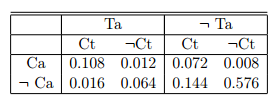
\includegraphics[scale=1]{resources/img3a.png}
			\caption{Probability Distribution Table}
		\end{center}
	\end{figure}

	Based on the given information, calculate the following. Show your computations.

	\begin{enumerate}
		\item
		P(Ta) \\
\begin{verbatim}
P(Ta) = 0.108 + 0.012 + 0.016 + 0.064
P(Ta) = 0.2
\end{verbatim}
		\textbf{P(Ta) = 0.2}

		\item
		P(Ca) \\
\begin{verbatim}
P(Ca) = 0.108 + 0.012 + 0.072 + 0.008
P(Ca) = 0.2
\end{verbatim}
		\textbf{P(Ca) = 0.2}
		\item
		P(Ta | Ca) \\
		\begin{equation*}
			\frac{P(Ta \cap Ca)}{P(Ca)}
		\end{equation*}
		\begin{equation*}
			\frac{.108 + .012}{.2}
		\end{equation*}
		\begin{equation*}
			\frac{.12}{.2}
		\end{equation*}
		\textbf{P(Ta | Ca) = 0.6}

		\item
		P(Ca | Ta $\vee$ Ct)
		\begin{equation*}
			\frac{P(Ca \cap (Ta \cup Ct))}{P(Ta \cup Ct)}
		\end{equation*}
		\begin{equation*}
			\frac{0.108 + 0.072 + .012}{0.108 + 0.012 + 0.016 + 0.064 + 0.072 + 0.144}
		\end{equation*}
		\begin{equation*}
			\frac{.18}{.416}
		\end{equation*}
		\textbf{P(Ca | Ta $\vee$ Ct) = 0.4615}
	\end{enumerate}

\end{document}